\section{Normalized Quantization-aware Training}



\begin{frame}{Quantization Error}
  Another significant bottleneck is the use of expensive \textbf{high-speed} and precision \textbf{analog-to-digital} and 
  \textbf{digital-to-analog} conversion modules\footnote{\scriptsize Tsakyridis, A., Moralis-Pegios, M., Giamougiannis, G., \textbf{Kirtas,
    M.}, Passalis, N., Tefas, A. and Pleros, N., 2024.
  \href{https://pubs.aip.org/aip/app/article/9/1/011102/3161086}{Photonic
  neural networks and optics-informed deep learning fundamentals.} APL
Photonics, 9(1).}.

\begin{center}
  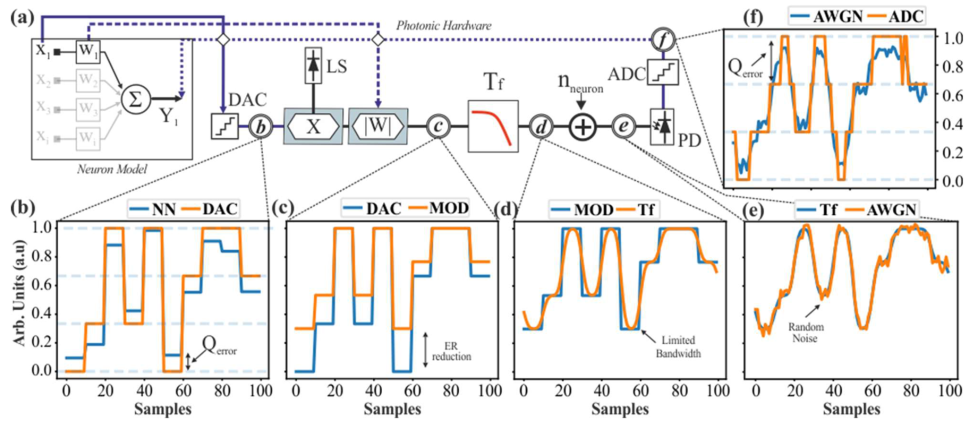
\includegraphics[width=0.8\linewidth]{sections/2_quant/imgs/apl_noise.png}  
\end{center}
  

  % This Chapter studies quantization phenomena in photonic models, induced by
  % DACs/ADCs, as an additional noise/uncertainty.

\end{frame}

% \begin{frame}{Contribution 2}
%   \textbf{(Contribution 2)}  A data driven quantization-aware training approach
%   that   
%   \begin{itemize}
%     \item Takes into account the distribution of parameters involved to the
%       decision of the networks
%     \item Eliminating the outliers
%       \item Reducing the quantization loss
%     \end{itemize}
%     Studied from the prospective of photonic hardware
%     \begin{itemize}
%       \item Taking into account DAC and ADC applied to the mechanism of neuron
%         (e.g. input, weight, activation)
%       \item Applying photonic-compliant uniform quantization to parameters
%       \end{itemize}
%      Allowing us to reduce the bit-resolution (< 8-bits) of DL models without significant
%      performance degradation.
% \end{frame}

%%%%%%%%%%%%%%%%%%%%%%%%%%%%%%%%%%%%%% NEW FRAME %%%%%%%%%%%%%%%%%%%%%%%%%%%%%%%%%%%%%%
\begin{frame}{Thesis contribution}
    \textbf{An activation-agnostic, quantization-aware training
      method}, oriented to PNNs. 
    \begin{itemize}
        \item \textcolor{mygreen}{Lower performance degradation when lower bit resolution applied} 
        \item \textcolor{mygreen}{Lower the hardware complexity and cost}
    \end{itemize}
    % Taking into account:
    % \begin{itemize}
    %     \item Quantization-errors occurred during training
    %     \item The distribution of parameters involved during training
    % \end{itemize}
    
    % \textbf{\textcolor{mygreen}{Motivated by the assumption that the weights
    %     involved in ANN inference follow a Gaussian distribution}} 
\end{frame}
%%%%%%% this assumption has 2 references, should we mention both or 1 is enough?
    
% \footnote{X. Glorot and Y. Bengio, “Understanding the difficulty of training
% deep feedforward neural networks,” in Proc. Int. Conf. on Artificial
% Intelligence and Statistics, 2010, pp. 249–256. 2, 3}


% %%%%%%%%%%%%%%%%%%%%%%%%%%%%%%%%%%%%%% NEW FRAME %%%%%%%%%%%%%%%%%%%%%%%%%%%%%%%%%%%%%%
% \begin{frame}{Quantization-aware Training}
%   Under the proposed quantization-aware training framework, \textbf{every signal
%     that is involved in the response of the \(i\)-th layer is first quantized in
%     a specific floating range} \([p^{(i)}_{min}, \dots ,p^{(i)}_{max}]\). 
% \begin{figure}
%   \centering
%     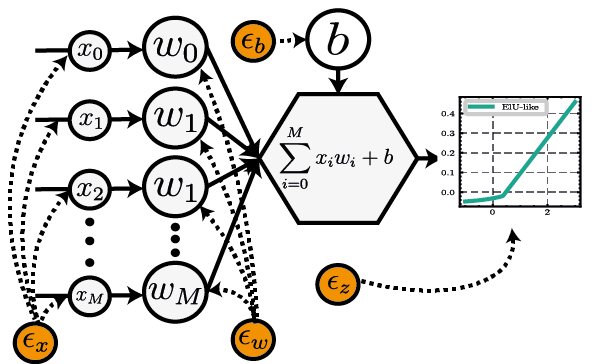
\includegraphics[width=0.65\linewidth]{sections/2_quant/imgs/quant_neuron.png}
% \end{figure}

% \textbf{During the evaluation, forward-pass quantization error \(\epsilon\) is injected by deploying the rounding of quantization arithmetically in floating point.}
% \end{frame}

% %%%%%%%%%%%%%%%%%%%%%%%%%%%%%%%%%%%%%% NEW FRAME %%%%%%%%%%%%%%%%%%%%%%%%%%%%%%%%%%%%%%
% \begin{frame}{Lower Bit Representation}
%   Under the proposed quantization-aware training framework, \textbf{every signal
%     that is involved in the response of the \(i\)-th layer is first quantized in
%     a specific floating range} \([p^{(i)}_{min}, \dots ,p^{(i)}_{max}]\) and they can be represented using \(B\) bits. 
    
%  First, \textbf{every signal} $p^{(i)}$ is \textbf{converted to a bit representation} by applying the function \( Q:\mathbb{R} \rightarrow \mathbb{N}\):
% \begin{equation}
%     p_{q}^{(i)} = Q(p^{(i)}, s_p^{(i)}, \zeta_p^{(i)}) =  clip \left\{\nint*{\frac{p^{(i)}}{s_p^{(i)}} + \zeta_{p}^{(i)}}, q_{min}, q_{max}\right\} \in \mathbb{N}
% \end{equation}
% {\scriptsize where \(p^{(i)} \in \mathbb{R}\), \(p_{q}^{(i)} \in [0\ldots, 2^B-1]\) and \(B\) denotes the bit resolution of the signal.}

% \textbf{Then, \(p_{q}^{(i)}\) is converted to discrete floating arithmetics} \(p_{q}^{(i)} \in [p^{(i)}_{min},  \ldots, p^{(i)}_{min}]\) using a dequantization function \(D: \mathbb{N} \rightarrow \mathbb{R}\):
% \begin{equation}
%     p_f^{(i)} = D(p^{(i)}_{q}, s_p^{(i)}, \zeta_p^{(i)}) = s_{p}^{(i)} (p_{q}^{(i)}-\zeta_{p}^{(i)}) \in \mathbb{R}
% \end{equation}

% \end{frame}

%%%%%%%%%%%%%%%%%%%%%%%%%%%%%%%%%%%%%% NEW FRAME %%%%%%%%%%%%%%%%%%%%%%%%%%%%%%%%%%%%%%
\begin{frame}{Quantization-aware Training}
The linear response of \(i\)-th layer is given by:
\begin{equation}
\bm{z}_{f}^{(i)} = Quant(\bm{W}_{f}^{(i)} \cdot \bm{y}_f^{(i-1)} + \bm{b}_f^{(i)}) \in \mathbb{R}^{N_i},
\end{equation}
{\scriptsize where \(Quant(\bm{x})\) denotes the process of quantization followed by dequantization of a vector or matrix \(\bm{x} \in \mathbb{R}^{M_i}\).}
\begin{center}
    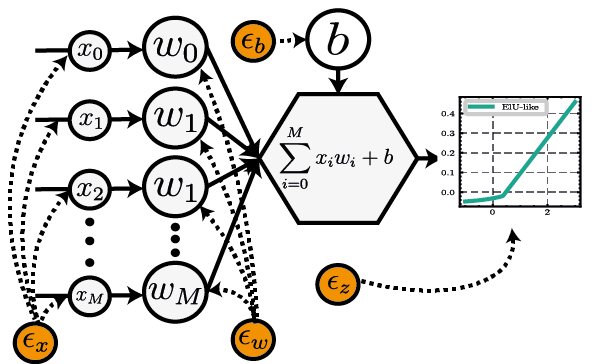
\includegraphics[width=0.6\linewidth]{sections/2_quant/imgs/quant_neuron.png}    
\end{center}
\begin{equation}
    \bm{y}^{(i-1)} = g^{(i)}((\bm{W}^{(i)} + \bm{\epsilon}_w) (\bm{y}^{(i-1)} + \bm{\epsilon}_y) + \bm{b}^{(i)} + \bm{\epsilon}_b) + \epsilon_g \in \mathbb{R}^{N_i}.
\end{equation}

% \textbf{The quantization error is propagated through the network} as a noise signal that is taken into account  \textbf{during training} affecting the overall performance of the network. 

% The output $\bm{z}_{f}^{(i)}$ passes through the photonic activation function, \(g(\cdot)\) of the neuron 
% \begin{equation}
%     \bm{y}^{(i)}_{f} = Quant(g( \bm{z}_{f}^{(i)})).
% \end{equation}
% \textbf{All signals involved in the layer's output are distributed in a uniform floating range between \(p_{min}^{(i)}\) and \(p_{max}^{(i)}\)} 
\end{frame}

% %%%%%%%%%%%%%%%%%%%%%%%%%%%%%%%%%%%%%% NEW FRAME %%%%%%%%%%%%%%%%%%%%%%%%%%%%%%%%%%%%%%
% \begin{frame}{Quantization-aware Training}


% % For example, for the weights $\bm{w}$, the quantization error is calculated as $\bm{\epsilon}_w = Quant(\mathbf{w}) - \mathbf{w}$.
% \end{frame}




%%%%%%%%%%%%%%%%%%%%%%%%%%%%%%%%%%%%%% NEW FRAME %%%%%%%%%%%%%%%%%%%%%%%%%%%%%%%%%%%%%%
\begin{frame}{Scaling Factor}
\tikzstyle{na} = [baseline=-.5ex]
\textbf{\textit{Scale}} defining the range of uniform bucket,
    \begin{equation}
        s^{(i)}_p= \frac{p^{(i)}_{max}-p^{(i)}_{min}}{q_{max}-q_{min}} \in \mathbb{R}^{+},
    \end{equation}
    {\scriptsize where \(q_{min}=0\) and \(q_{max} = 2^B-1\) denote the range of an \(B\)-bit resolution.}

    \begin{center}
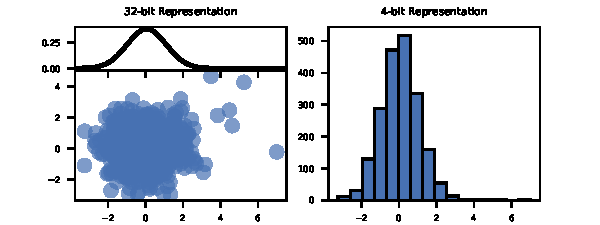
\includegraphics[\width=\linewidth]{sections/2_quant/imgs/motivation_1.pdf}    
\end{center}
\textbf{Effective range, i.e.,  minimum (\(p^{(i)}_{max} \in \mathbb{R}\)) and maximum (\(p^{(i)}_{min} \in \mathbb{R}\)) values} affects the amount of quantization error.

    % (0 and \(\) respectively) while \(p^{(i)}_{max} \in \mathbb{R}\) and \(\) represents the working range, i.e., maximum and minimum, of a signal.
    

% \textbf{Zero-point is a low precision value that represents the quantized value that will represent the real value 0}, and it is calculated as: 
% \begin{equation}
% \zeta_p^{(i)} = clip\left\{ \nint*{q_{min} - \frac{p^{(i)}_{min}}{s^{(i)}_p}} , q_{min}, q_{max}\right\} \in \mathbb{N}    
% \end{equation}

\end{frame}


% %%%%%%%%%%%%%%%%%%%%%%%%%%%%%%%%%%%%%% NEW FRAME %%%%%%%%%%%%%%%%%%%%%%%%%%%%%%%%%%%%%%
% \begin{frame}{Working Range}
%  \vspace{5pt}
%  % in inference, \textbf{is the selected working range, i.e.,  minimum (\(p_{min}\)) and maximum (\(p_{max}\)) values}, of a signal on which the scale of uniform buckets depends. 
% \end{frame}

% %%%%%%%%%%%%%%%%%%%%%%%%%%%%%%%%%%%%%% NEW FRAME %%%%%%%%%%%%%%%%%%%%%%%%%%%%%%%%%%%%%%
% \begin{frame}{Normalized Quantization}
% %  Assuming that every signal involved in the response of each
% % neuron follows a \textbf{Gaussian distribution,  i.e.,  \(p \sim \mathcal{N}(\mu, \sigma)\):}


% \textbf{The proposed method is more robust to outliers}
% \end{frame}

\begin{frame}{Normalized Quantization}
    Quantization is applied using the \textit{proxy} minimum and maximum.
\begin{gather}
\label{eq:proposed_statistics}
    p_{min} = \tilde{\mu}^{p}_{K} - \alpha\tilde{\sigma}^{p}_{K} \in \mathbb{R},  \text{   }
    p_{max} = \tilde{\mu}^{p}_{K} + \alpha\tilde{\sigma}^{p}_{K} \in \mathbb{R}.
\end{gather}


% {\scriptsize where \textbf{$\alpha$}  denotes the scaling factor that
% controls the coverage used of the estimated normal distribution.}
\begin{center}
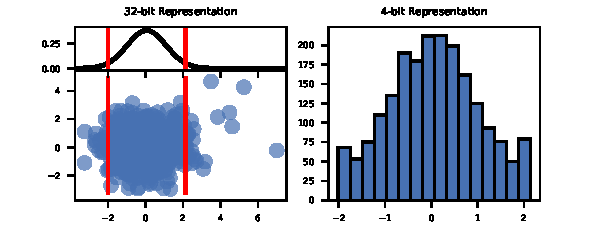
\includegraphics[\width=\linewidth]{sections/2_quant/imgs/motivation_2.pdf}    
\end{center}
Scaling factor $\alpha \in \mathbb{R}$ adjusts the coverage of the density area of the distribution according to the applied bit resolution.

Quantized parameters range \([\mu - \alpha\sigma^2, \ldots, \mu+\alpha\sigma^2] \in \mathbb{R}^N\) maintaining the \textbf{ maximum information at distribution's high density area}.
\end{frame}

% %%%%%%%%%%%%%%%%%%%%%%%%%%%%%%%%%%%%%% NEW FRAME %%%%%%%%%%%%%%%%%%%%%%%%%%%%%%%%%%%%%%
% \begin{frame}{Normalized Quantization Post training parameters}
% \begin{itemize}
%     \item 
% The probability of a normal deviation lies in the range \([\mu - \alpha\sigma, \mu + \alpha\sigma]\), based on the 68–95–99.7 rule, given by:
% \end{itemize}
% \begin{equation}
%      F(\mu +\alpha\sigma )-F(\mu -\alpha\sigma )= erf\left({\frac {\alpha}{\sqrt {2}}}\right) \in \mathbb{R},
% \end{equation}
% where \(F(\cdot)\) is the general form of the probability density function and \(erf(x)=\frac{2}{\sqrt{\pi}}\int_0^x e^{t^2}dt \) denotes the Gauss error function.
% \end{frame}

%%%%%%%%%%%%%%%%%%%%%%%%%%%%%%%%%%%%%% NEW FRAME %%%%%%%%%%%%%%%%%%%%%%%%%%%%%%%%%%%%%%
\begin{frame}{Estimated Parameters Distribution}
    Since the distribution of parameters is transformed during the training, the proposed method \textbf{progressively estimates} the distribution in every epoch by \textbf{applying an exponential moving average}.
\begin{gather}
    \label{eq:proposed_collection}
    \tilde{\mu}^{p}_{t} = \beta  E[\bm{p}_t] + (1 - \beta) \tilde{\mu}^{p}_{t-1} \in \mathbb{R}, \\
    \tilde{\sigma}^{p}_{t} = \beta Var[\bm{p}_t]^{1/2} + (1 - \beta) \tilde{\sigma}^{p}_{t-1} \in \mathbb{R},
\end{gather}
{\scriptsize where \(t = 1 \ldots K\), \(K \in \mathbb{N}\) denotes the number of epochs, and $\beta \in \mathbb{R}$ is a weighting parameter of the exponential average.}

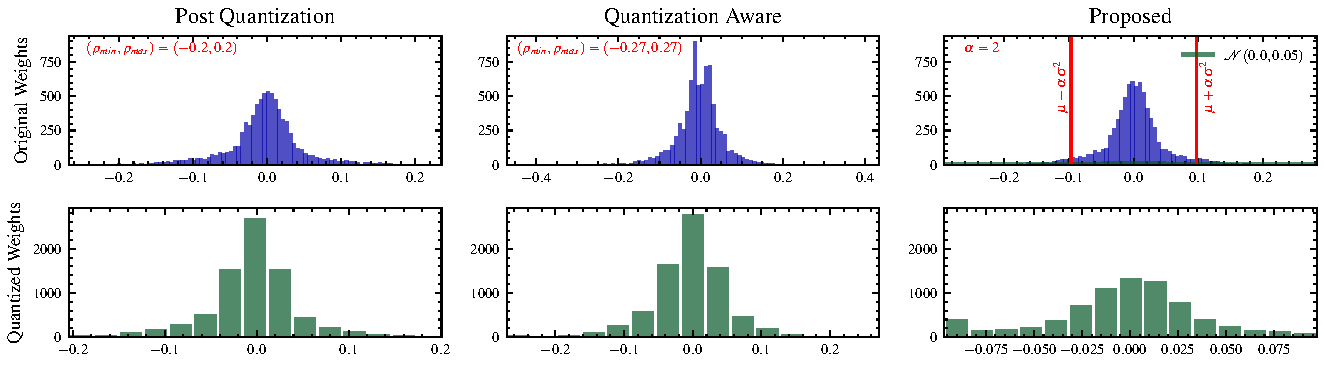
\includegraphics[width=\linewidth ]{sections/2_quant/imgs/mnist_histograms_layer_00.pdf}

\end{frame}



%%%%%%%%%%%%%%%%%%%%%%%%%%%%%%%%%%%%%% NEW FRAME %%%%%%%%%%%%%%%%%%%%%%%%%%%%%%%%%%%%%%
\begin{frame}{Quantization-aware \& Post Training Quantization}
\begin{center}
    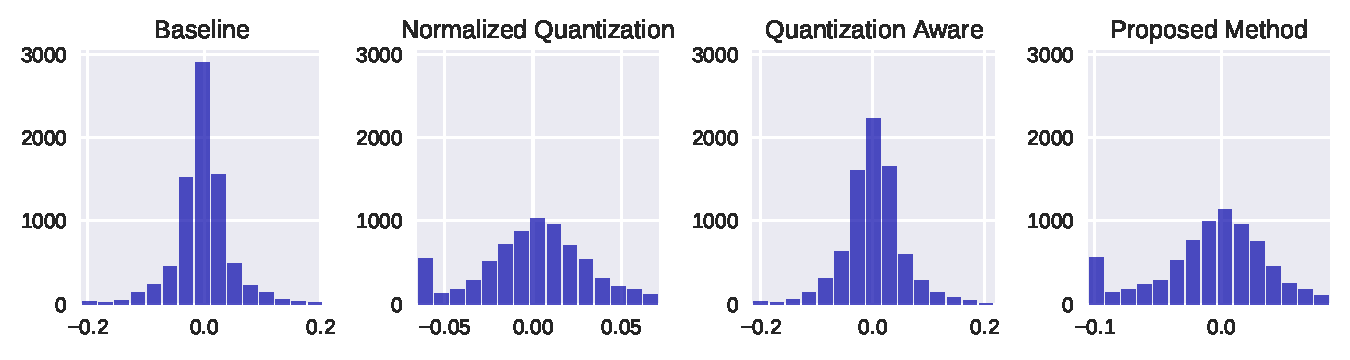
\includegraphics[width=\linewidth]{sections/2_quant/imgs/mnist_histograms_layer_0.pdf}
\end{center}

\textbf{Normalized-quantization can be used both in post training and quantization-aware training.}
\end{frame}

\begin{frame}{The Role of Coverage}
    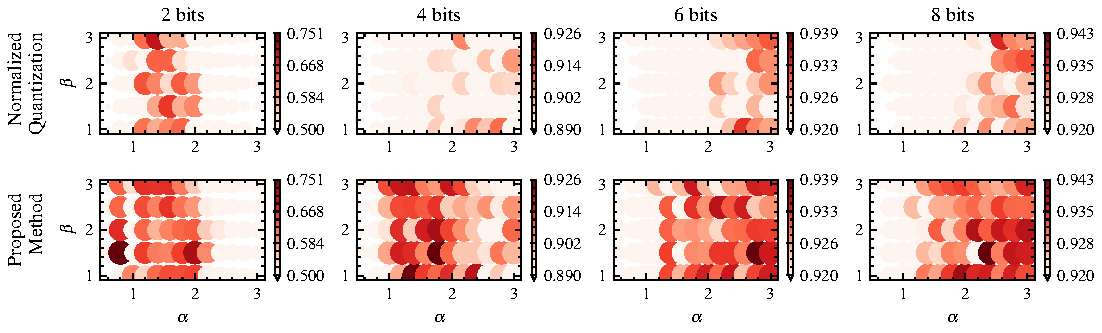
\includegraphics[width=\linewidth]{sections/2_quant/imgs/mnist_alpha_beta_plt.pdf}
    \begin{itemize}
        \item Intensity represents higher accuracy
        \item The normalized quantization do not highly depends on weighting parameter of the exponential average
        \item Tuning of scaling factor $\alpha \in \mathbb{R}$ should consider the applied bit resolution 
    \end{itemize}
\end{frame}



% \begin{frame}{Image Classification using FCNN}
% \begin{table}[h]
% \caption{Evaluating the proposed method on the MNIST dataset using a fully connected architecture (classification accuracy (\%) is reported).}
% \label{table:eval_mnist}
% \centering
% \resizebox{\linewidth}{!}{
% \begin{tabular}{l|cccc}
%     \toprule
%       \textbf{Bits} &  \textbf{Post Quant.} & \textbf{Norm. Post Quant.} & \textbf{Quant-aware Training} & \textbf{Proposed} \\
%      \midrule
%      \multicolumn{5}{c}{\textbf{Photonic Sinusoidal}}\\
%      \midrule
%      8 & $90.12 \pm{1.52}$ & $91.46 \pm 0.22$ & $91.21 \pm{0.49}$ & $\textbf{91.65} \pm \textbf{0.12}$\\
%      6 & $86.93 \pm{1.47}$ & $91.15 \pm 0.71$ & $91.04 \pm{0.51}$ & $\textbf{91.67} \pm \textbf{0.49}$\\
%      4 & $0.09 \pm{0.46}$ & $87.28 \pm 0.84$ & $90.26 \pm{0.77}$ & $\textbf{90.68} \pm \textbf{1.41}$\\
%      2 &  $0.09 \pm{0.26}$ & $66.36 \pm 4.53$ & $67.63 \pm{2.28}$ & $\textbf{79.31} \pm \textbf{2.06}$ \\
%      \midrule
%      \multicolumn{5}{c}{\textbf{Photonic Sigmoid}}\\
%      \midrule
%       8 & $91.02 \pm{0.81}$ & $91.81 \pm 0.36$ & $91.17 \pm{0.33}$ & $\textbf{91.79} \pm \textbf{0.25}$ \\
%       6 & $87.01 \pm{0.12}$ & $91.79 \pm 0.61$ & $91.02 \pm{0.29}$ & $\textbf{91.31} \pm \textbf{0.55}$ \\
%       4 & $0.09 \pm{0.25}$ & $87.14 \pm 0.21$ & $90.22 \pm{0.39}$ & $\textbf{90.76} \pm \textbf{0.37}$ \\
%       2 & $0.09 \pm{0.23}$ & $64.22 \pm 0.47$ & $61.26 \pm{1.95}$ & $\textbf{75.04} \pm \textbf{3.56}$\\
%      \bottomrule
% \end{tabular}}
% \label{tab:mnist_exp}
% \end{table}
% \end{frame}

%\subsection*{Image Classification using CNN}
\begin{frame}{Image Classification using CNNs}
\begin{table}[h]
\caption{Evaluating the proposed method on the CIFAR10 dataset using a convolutional architecture (classification accuracy (\%) is reported).}
\label{table:eval_cifar10}
\centering
\resizebox{\linewidth}{!}{
\begin{tabular}{l|cccc}
    \toprule
         \textbf{Bits} &  \textbf{Post Quant.} & \textbf{Norm. Post Quant.} & \textbf{Quant-aware Training} & \textbf{Proposed} \\
     \midrule
     \multicolumn{5}{c}{\textbf{Photonic Sinusoidal}}\\
     \midrule
     8 & $15.22 \pm{1.15}$ & $68.22 \pm 1.58$ & $67.64 \pm{1.24}$ & $\textbf{80.08} \pm \textbf{0.63}$\\
     6 & $15.10 \pm{1.81}$ & $63.61 \pm 0.79$ & $66.56 \pm{1.38}$ & $\textbf{77.81} \pm \textbf{0.43}$\\
     4 & $16.62 \pm{2.44}$ & $60.89 \pm 5.84$ & $29.48 \pm{10.43}$ & $\textbf{76.77} \pm \textbf{0.58}$\\
    %  2 &  $ \pm{}$ & $ \pm{} $ & $ \pm{}$ & $\textbf{} \pm \textbf{}$ \\
     \midrule
     \multicolumn{5}{c}{\textbf{Photonic Sigmoid}}\\
     \midrule
      8 & $16.39\pm{1.15}$ & $55.22 \pm 3.07$ & $66.23 \pm{1.23}$ & $\textbf{72.36} \pm \textbf{0.71}$ \\
      6 & $15.76 \pm{0.73}$ & $54.62 \pm 2.39$ & $66.56 \pm{1.61}$ & $\textbf{72.22} \pm \textbf{1.29}$ \\
      4 & $16.38 \pm{0.25}$ & $44.21 \pm 6.44$ & $65.25 \pm{1.96}$ & $\textbf{71.56} \pm \textbf{0.58}$ \\
    %   2 & $ \pm{}$ & $ \pm $ & $ \pm{}$ & $\textbf{} \pm \textbf{}$\\
     \bottomrule
\end{tabular}}
\label{table:3}
\end{table}
\end{frame}


%\subsection*{Image Classification using CNN}

% \textbf{\begin{frame}{Focasting using RNN}
%   \begin{table}
%     \caption{Evaluating the proposed method on the FI-2010 dataset using a recurrent architecture (Cohen's $\kappa$  is reported).}
%     \label{table:eval_fi2020}
%     \centering
%     \resizebox{\linewidth}{!}{
%       \begin{tabular}{l|cccc}
%         \toprule
%         \textbf{Bits} &  \textbf{Post Quant.} & \textbf{Norm. Post Quant.} & \textbf{Quant-aware Training} & \textbf{Proposed} \\
%         \midrule
%         \multicolumn{5}{c}{\textbf{Photonic Sinusoidal}}\\
%         \midrule
%         8 & $0.0502 \pm{0.0218}$ & $0.0840 \pm 0.0067$ & $0.1189 \pm{0.0105}$ & $\textbf{0.1347} \pm \textbf{0.0074}$\\
%         6 & $0.0647 \pm{0.0015}$ & $0.0825 \pm 0.0074$ & $0.1170 \pm{0.0115}$ & $\textbf{0.1342} \pm \textbf{0.0055}$\\
%         4 & $0.0645 \pm{0.0057}$ & $0.0756 \pm 0.0109$ & $0.1091 \pm{0.0210}$ & $\textbf{0.1184} \pm \textbf{0.0043}$\\
%         2 & $0.0370 \pm{0.0069}$ & $0.0416 \pm 0.0113$ & $0.0601 \pm{0.0031}$ & $\textbf{0.0782} \pm \textbf{0.0113}$\\
%         \midrule
%         \multicolumn{5}{c}{\textbf{Photonic Sigmoid}}\\
%         \midrule
%         8 & $0.0653 \pm{0.0081}$ & $0.0912 \pm 0.0085$ & $0.1262 \pm{0.0072}$ & $\textbf{0.1321} \pm \textbf{0.0024}$\\
%         6 & $0.0656 \pm{0.0061}$ & $0.0842 \pm 0.0042$ & $0.1242 \pm{0.0132}$ & $\textbf{0.1342} \pm \textbf{0.0052}$\\
%         4 & $0.0648 \pm{0.0062}$ & $0.0810 \pm 0.0062$ & $0.1232 \pm{0.0517}$ & $\textbf{0.1234} \pm \textbf{0.0039}$\\
%         2 & $0.0377 \pm{0.0126}$ & $0.0421 \pm 0.0032$ & $0.0918 \pm{0.0033}$ & $\textbf{0.0921} \pm \textbf{0.0014}$\\
%         \bottomrule
%       \end{tabular}}
% \end{table}
% \end{frame}
}
\begin{frame}{Deep Reinforcement Learning Evaluation - CartPole Task}
  \begin{figure}
     \centering
          \begin{subfigure}[b]{0.39\textwidth}
         \centering
         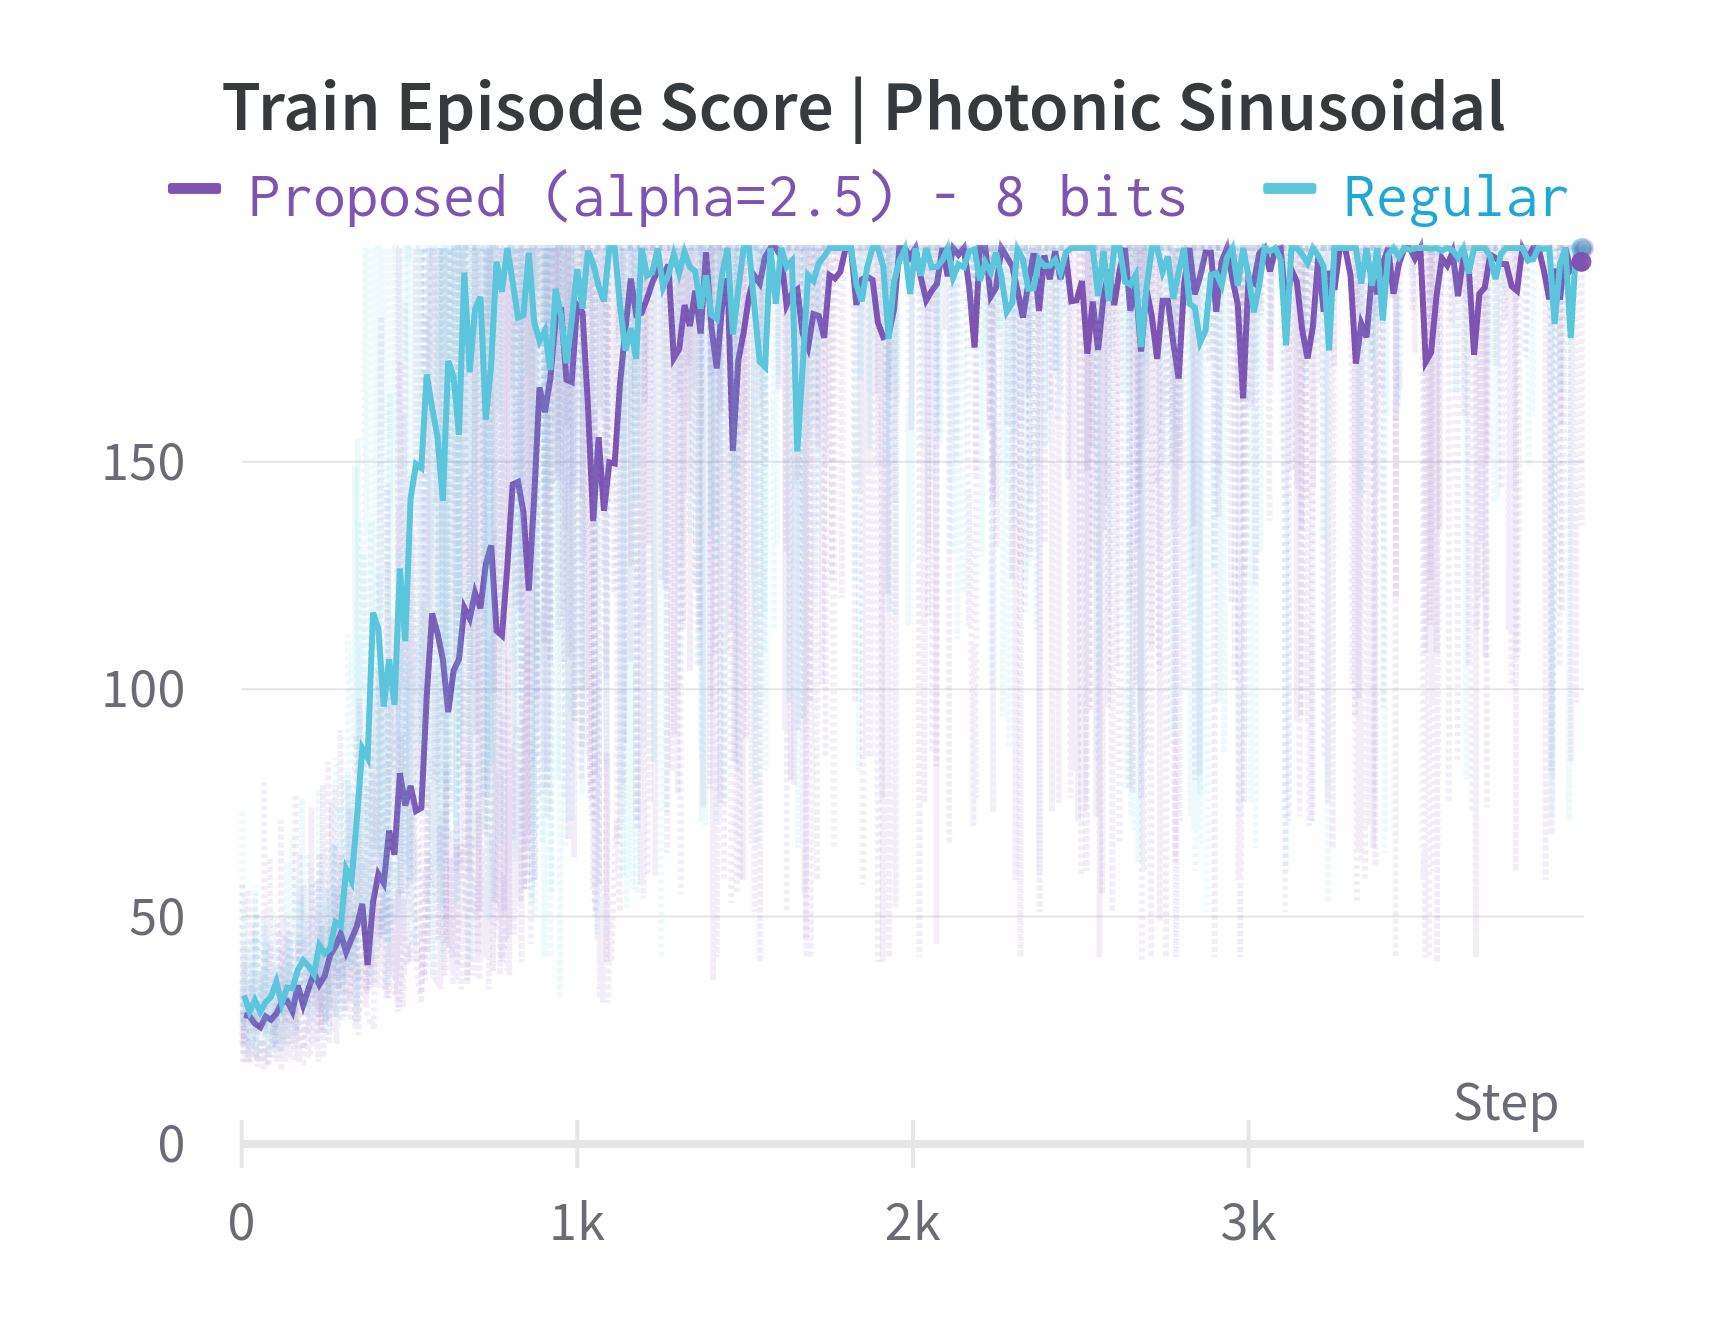
\includegraphics[width=\textwidth]{sections/2_quant/imgs/photonic_sinusoidal_8bits.png}
     \end{subfigure}
    \begin{subfigure}[b]{0.39\textwidth}
    \centering
    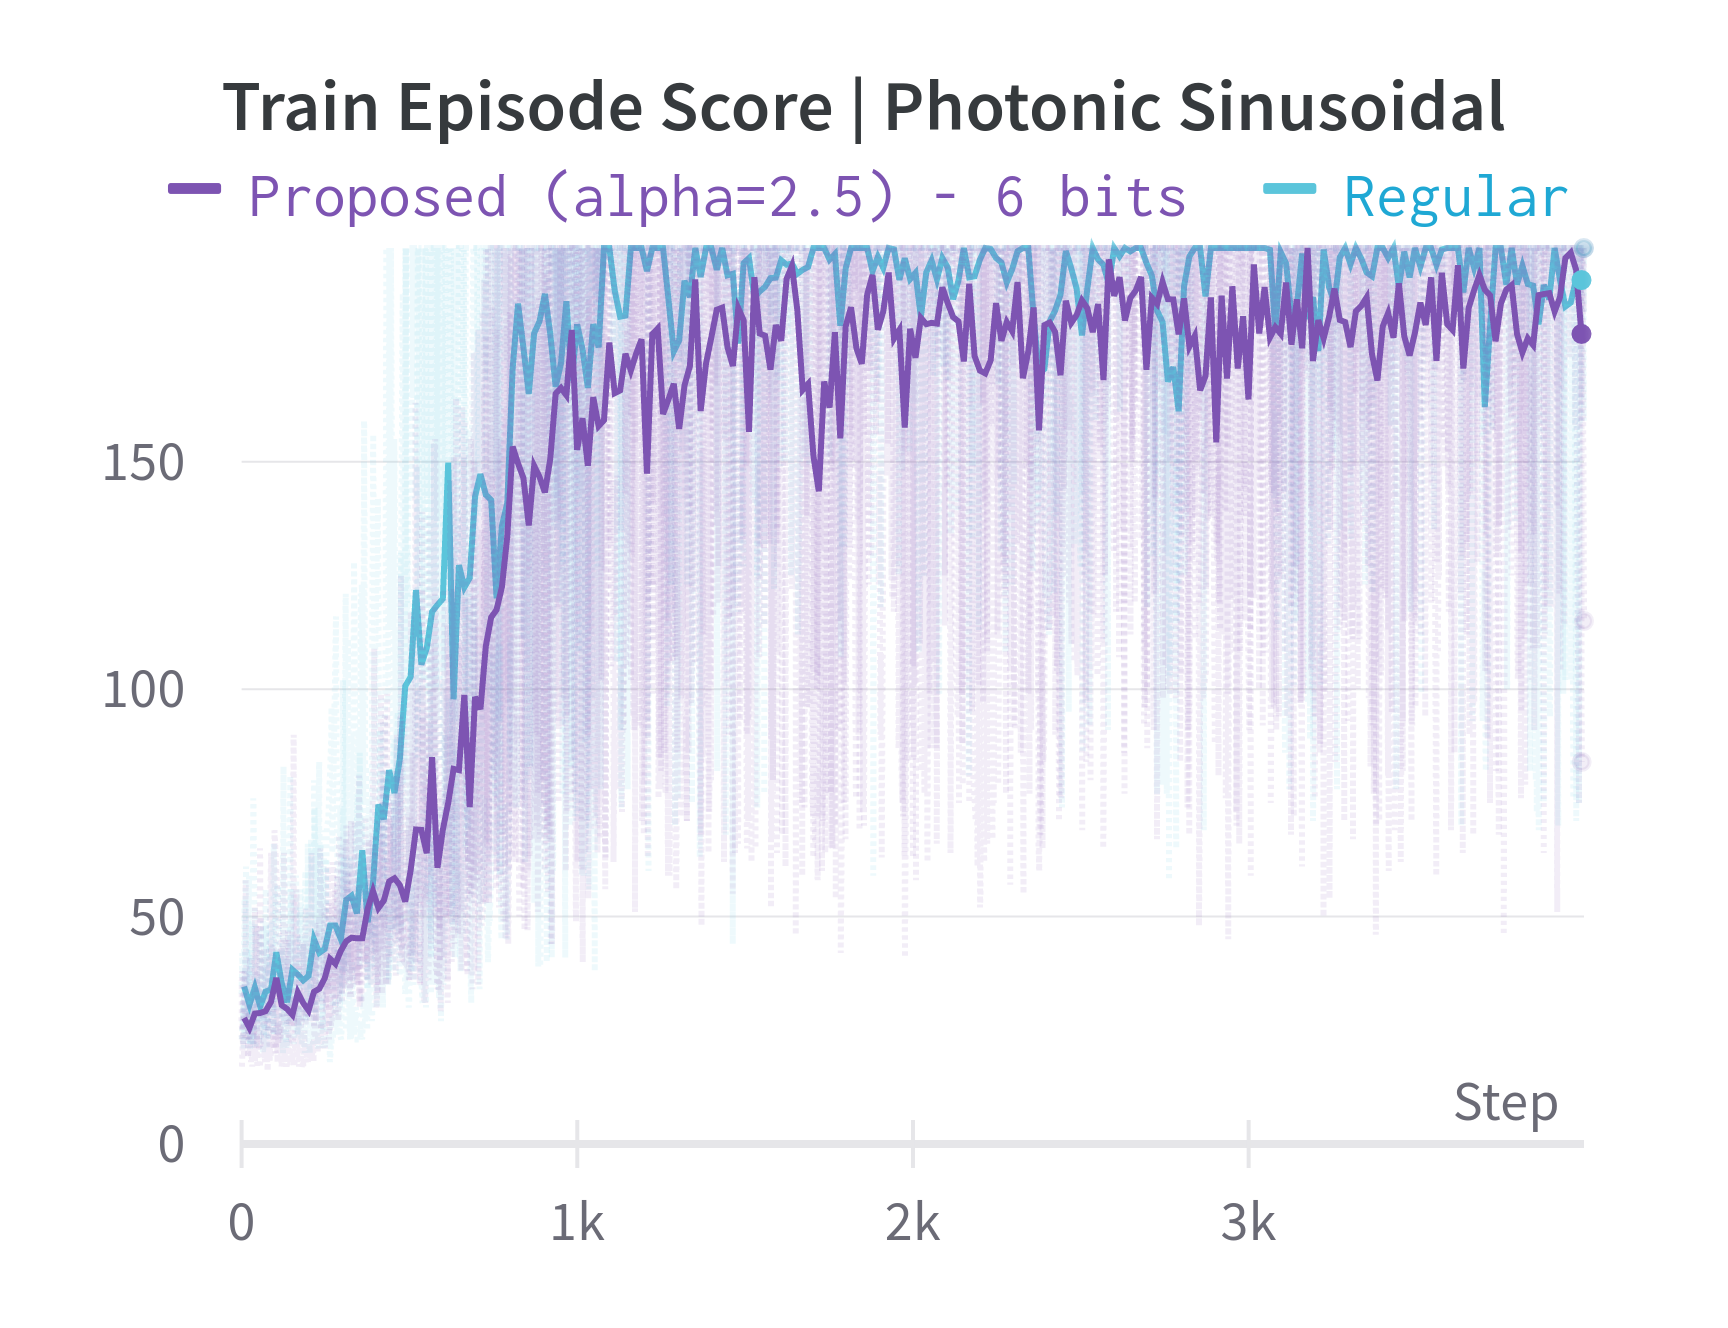
\includegraphics[width=\textwidth]{sections/2_quant/imgs/photonic_sinusoidal_6bits.png}
    \end{subfigure}\\
     \begin{subfigure}[b]{0.39\textwidth}
         \centering
         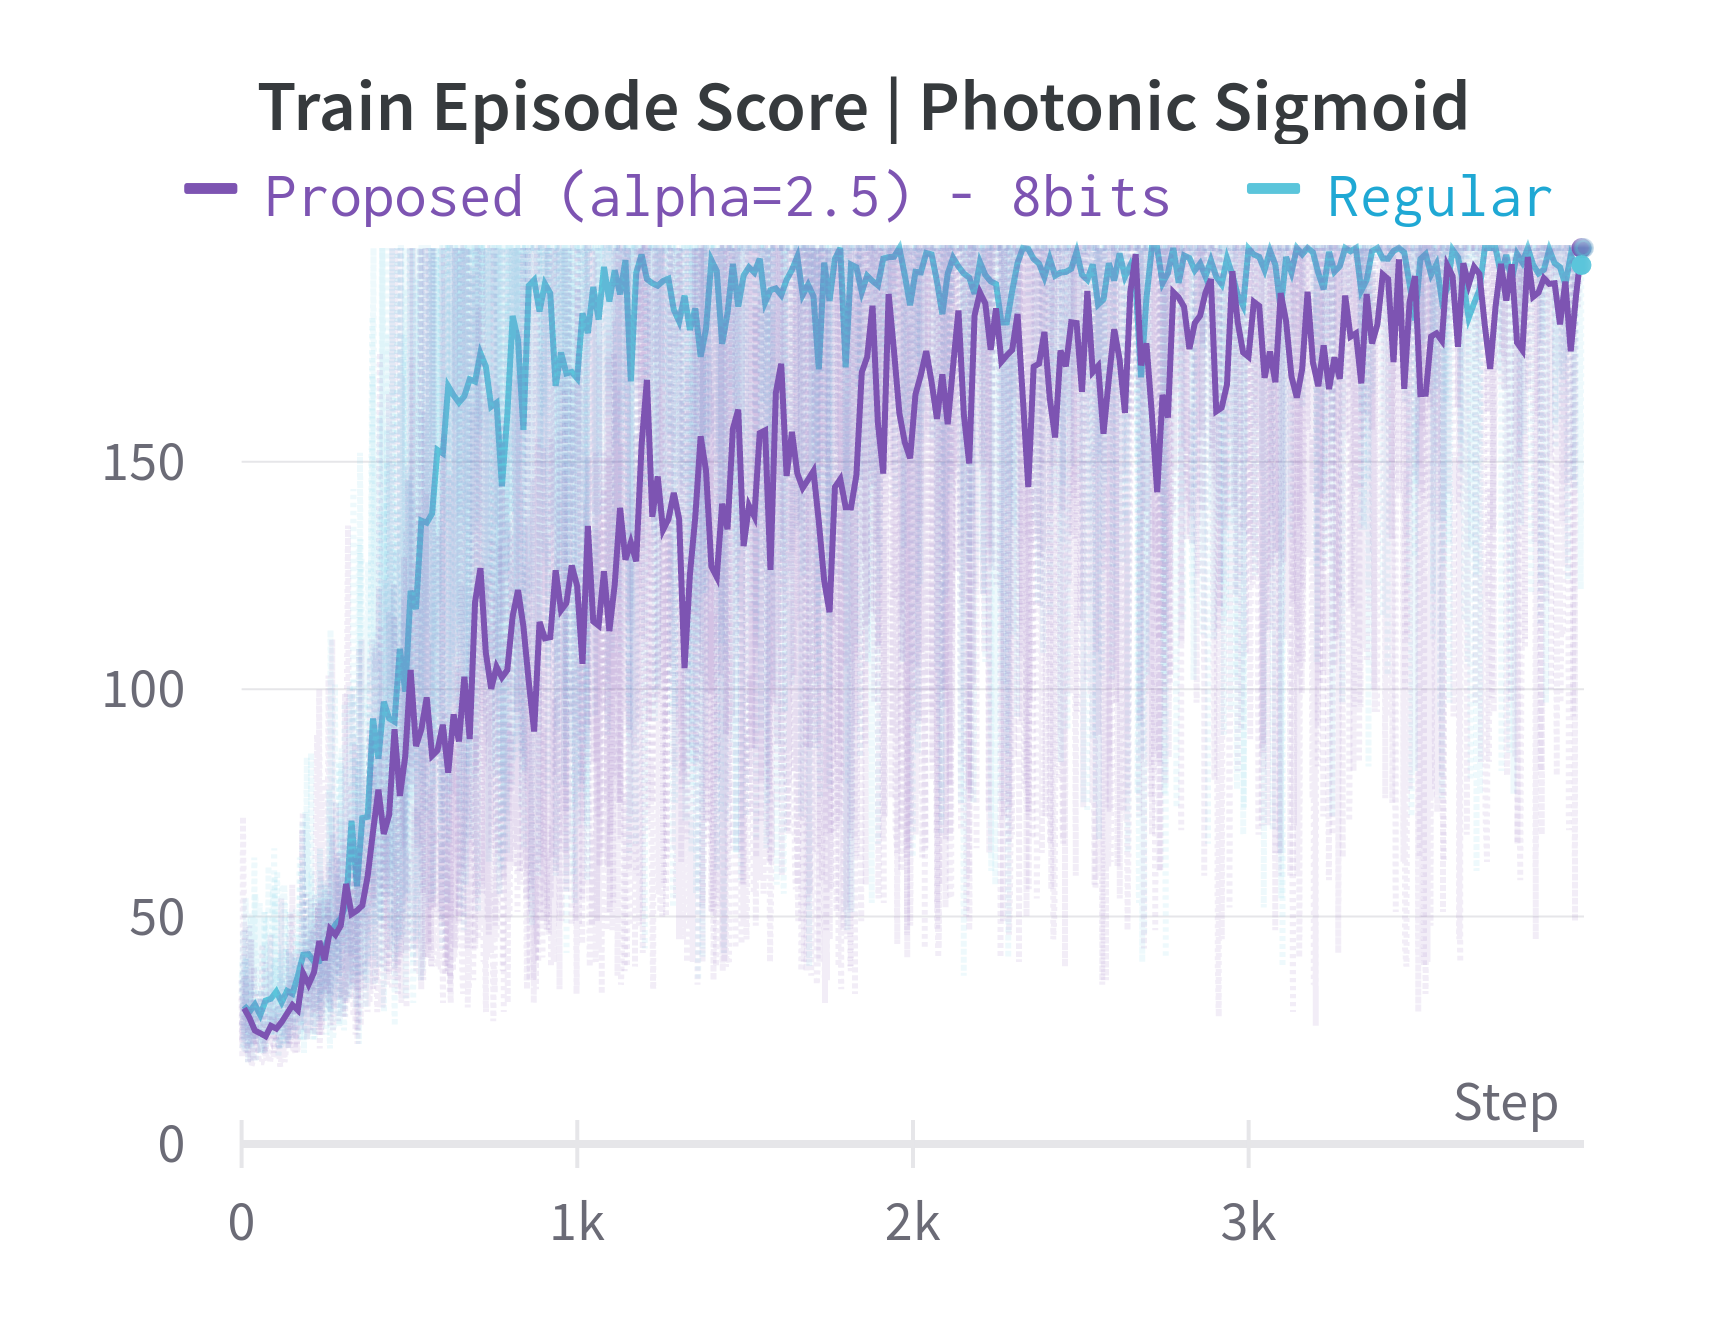
\includegraphics[width=\textwidth]{sections/2_quant/imgs/photonic_sigmoid_8bits.png}
     \end{subfigure}
     \begin{subfigure}[b]{0.39\textwidth}
         \centering
         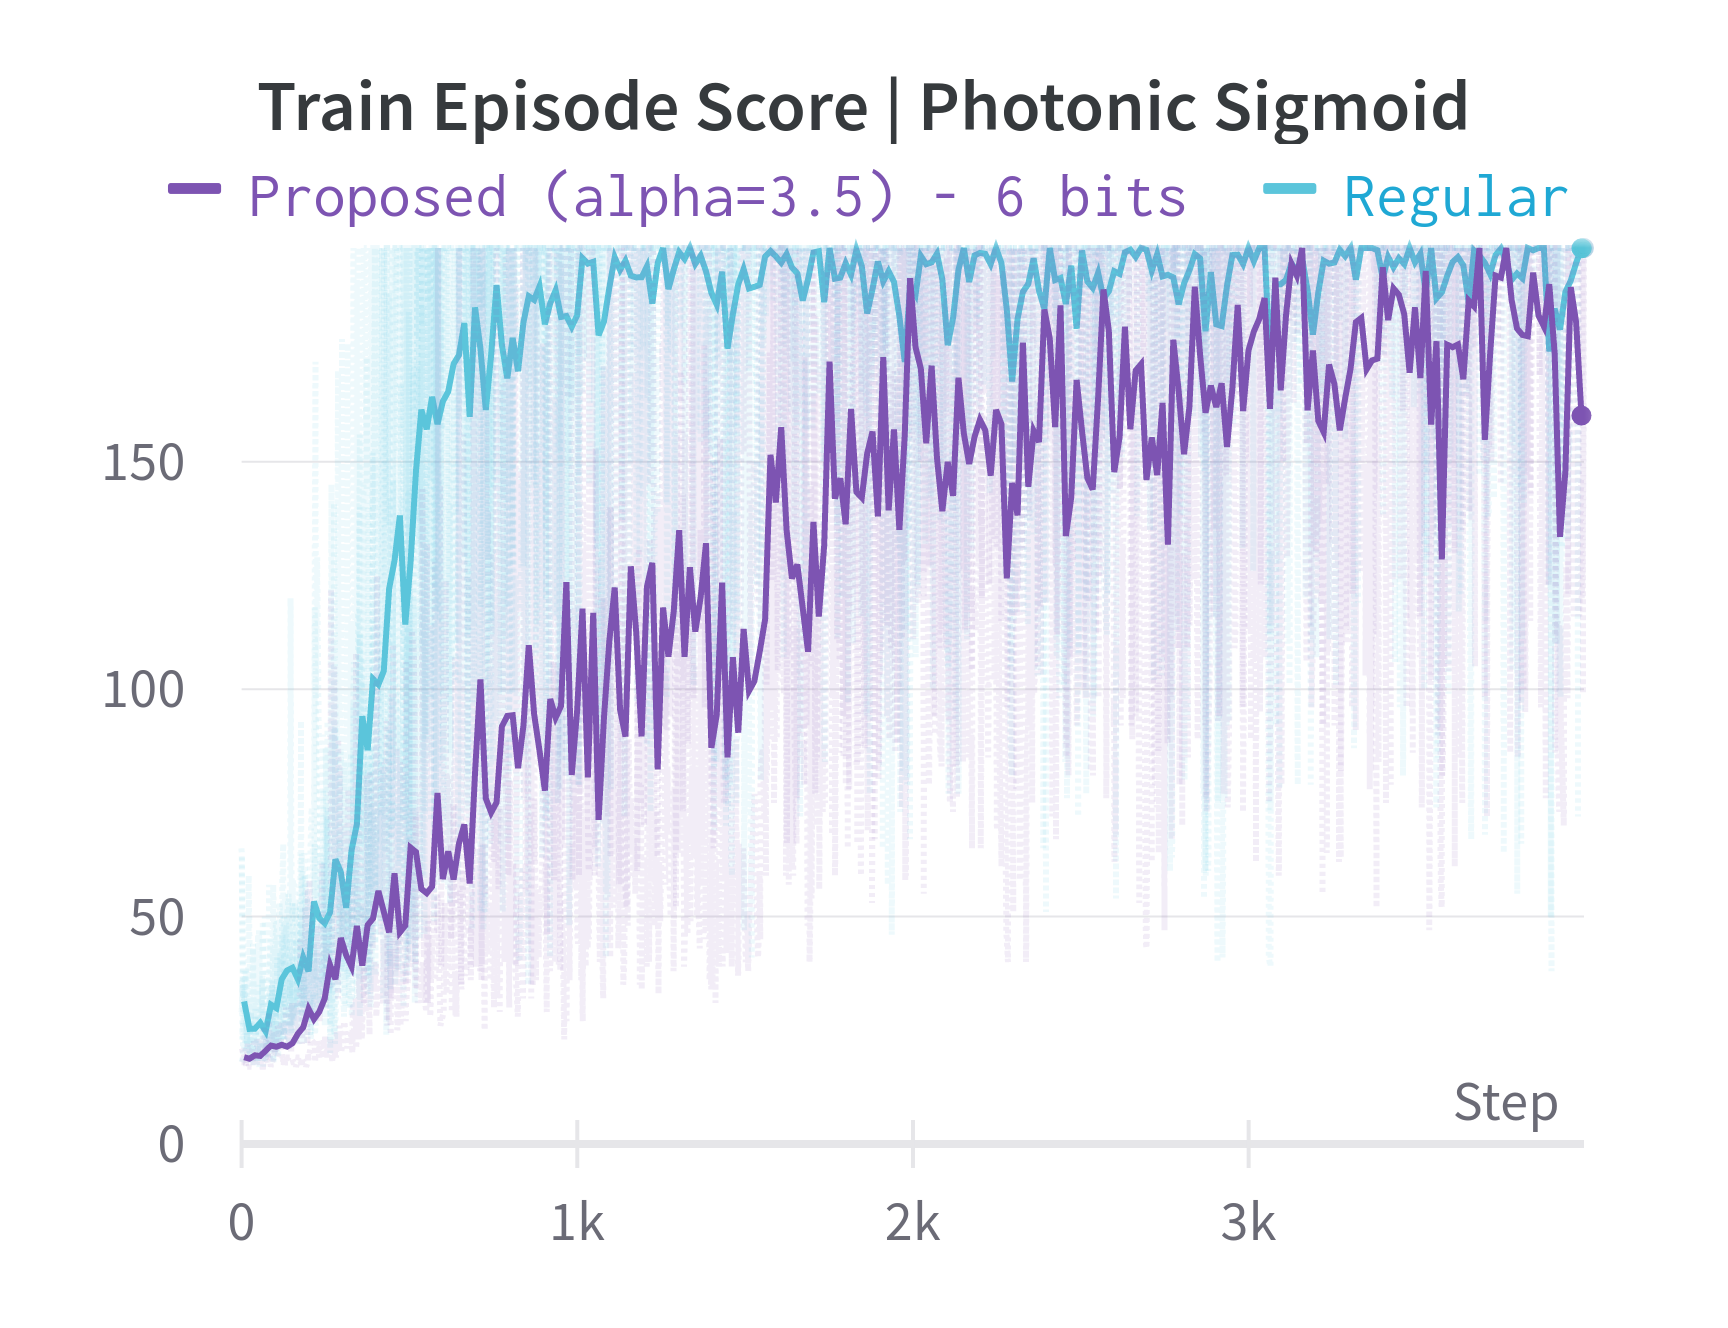
\includegraphics[width=\textwidth]{sections/2_quant/imgs/photonic_sigmoid_6bits.png}
     \end{subfigure}
    \caption{Average episode reward for each step obtained by the proposed method and regular (full resolution) training.}
    \label{fig:drl}
\end{figure}
\end{frame}

\begin{frame}{Publications}
\begin{itemize}
    \item Main Journal Publications
    \begin{itemize}
        \item {\scriptsize \textbf{Kirtas, M.}, Oikonomou, A., Passalis, N., Mourgias-Alexandris,
      G., Moralis-Pegios, M., Pleros, N. and Tefas, A., 2022. \href{https://www.sciencedirect.com/science/article/pii/S0893608022003598}{Quantization-aware training for low precision photonic neural networks.} Neural Networks, Elsevier}
    \end{itemize}
    \item Main Conference Publications 
        \begin{itemize}
        \item {\scriptsize \textbf{Kirtas, M.}, Passalis, N., Oikonomou, A., Mourgias-Alexandris, G., Moralis-Pegios, M., Pleros, N. and Tefas, A., 2022, December.\href{https://ieeexplore.ieee.org/abstract/document/10022168}{Normalized Post-training Quantization for Photonic Neural Networks.} In 2022 IEEE Symposium Series on Computational Intelligence (SSCI)} 
    \end{itemize}
\end{itemize}
\end{frame}

